%%%%%%%%%%%%%%%%%%%%%%%%%%%%%%%%%%%%%%%%%%%%%%%%%%%%%%%%%%%%%%%%%%
\subsection{Support Vector Machines (\acrshort{svm})}
\label{sec:svm}

\subsubsection{Puntuación de características}
\label{sec:svm1}

Para la técnica de \gls{svm}, también se procede a desarrollar una primera versión del clasificador para poder visualizar la importancia que toman cada una de las características en el mismo. En este caso, se trata de la clase \textit{SVC()} \cite{svc} y se inicializa un objeto de la misma con la definición por defecto de un kernel radial o gaussiano (\gls{rbf}), ya que se trabaja con un conjunto de datos no linearmente separables y que resulta complejo de operar si no se aumenta la dimensionalidad del espacio (ver Sección \ref{sec:mlsvm}). De la misma forma, \textit{SVC()} determina valores por defecto de los hiperparámetros \textit{C} y \textit{gamma}, que hacen referencia respectivamente, a la regularización del modelo y al impacto que produce cada instancia de entrenamiento en el proceso de clasificación. 

\vspace{3mm}

\begin{lstlisting}[style=Python, caption={Clasificador SVM por defecto}]
  classifier = SVC(kernel = 'rbf', random_state = 0) #por defecto C=1, gamma='scale' o 'auto'
  classifier.fit(X_train, y_train)
\end{lstlisting}
  
\vspace{3mm}

Cabe destacar que el proceso de ejecución y entrenamiento del clasificador del \gls{svm} a partir del conjunto de datos presenta una duración mucho mayor que el \gls{rf}. No obstante, una vez finaliza, se le aplican dos métodos de puntuación de características. Por un lado, se estima la importancia de las características a partir de la distancia que tienen hacia los vectores de soporte. En este caso es preciso basarse en los atributos \textit{support\_vectors\_} y \textit{dual\_coef\_}, que proporcionan la información sobre los vectores soporte que se han definido en el \gls{svm} y los multiplicadores de \textit{Lagrange} asociados. El resultado se expone en la Figura \ref{fig:imp3}, en la cual se visualiza cómo las longitudes de las etiquetas origen y destino inciden en la clasificación significativamente, ya que el resto de características tienen puntuaciones mucho más bajas.

\vspace{3mm}

\begin{figure}[H]
    \centering
    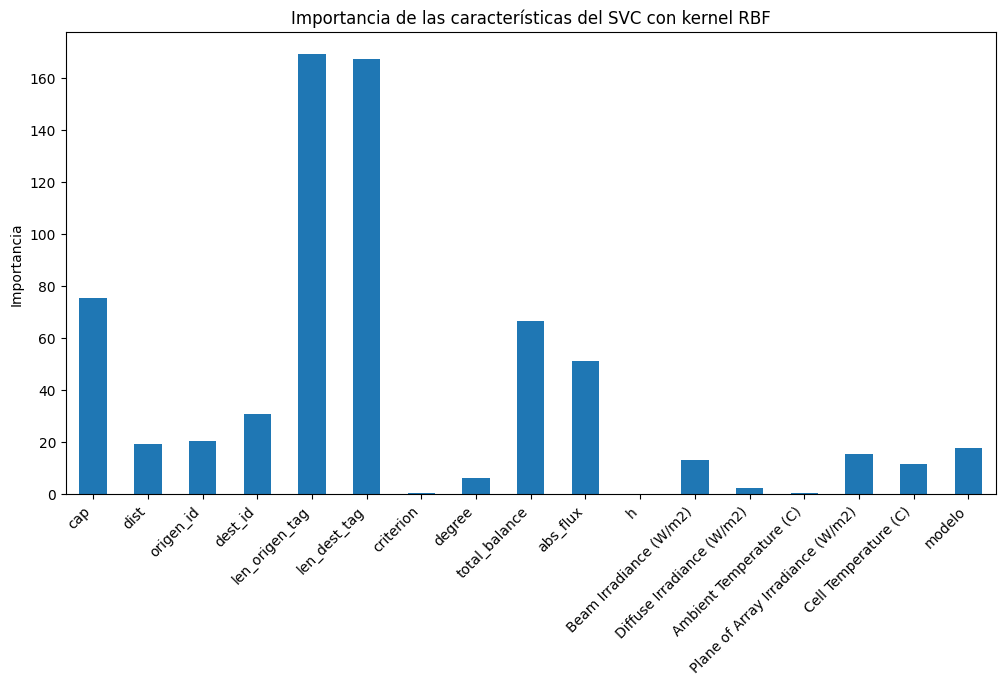
\includegraphics[width=1\textwidth]{img/desarrollo/svm/importance3.png}
    \caption{Puntuación de características del \acrshort{svm} mediante los atributos \textit{support\_vectors\_} y \textit{dual\_coef\_}}
    \label{fig:imp3}
\end{figure}

\vspace{3mm}

Por otro lado, al igual que se ha expuesto para el \gls{rf} (ver Sección \ref{sec:rf1}), se incluye el análisis a partir del método de la permutación (\textit{permutation\_importance}). En este caso, las longitudes de las etiquetas siguen siendo predominantes, pero las características que hacen referencia a la capacidad y al flujo total de energía resultante de \gls{den2ne} (\textit{abs\_flux}) también presentan valores de puntuaciones a considerar.

\begin{figure}[H]
    \centering
    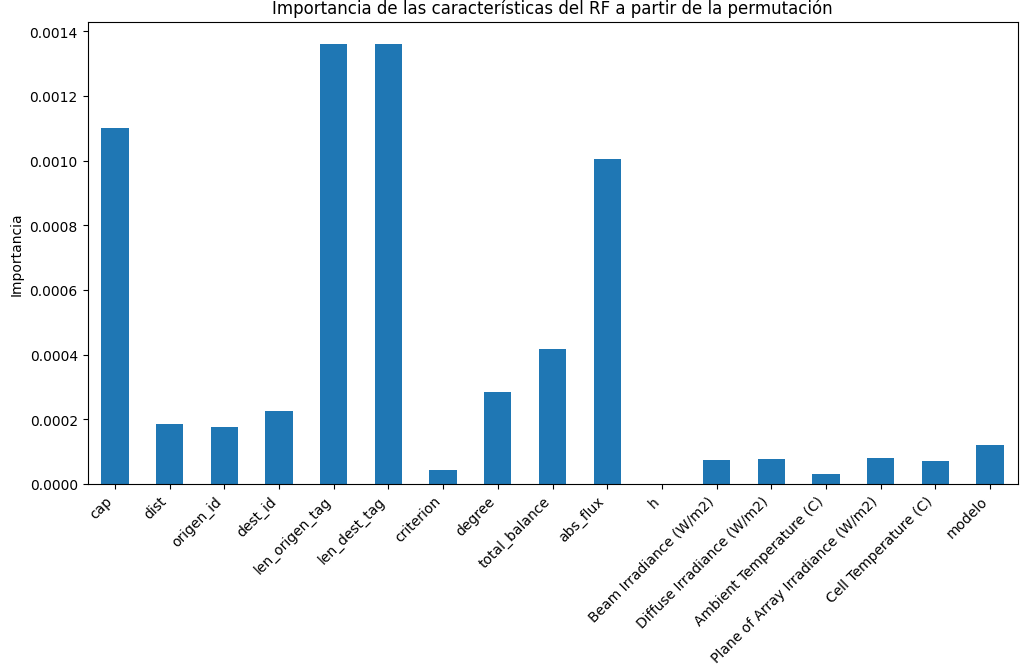
\includegraphics[width=1\textwidth]{img/desarrollo/svm/importance4.png}
    \caption{Puntuación de características del \acrshort{svm} mediante el método \textit{permutation\_importance}}
    \label{fig:imp4}
\end{figure}

\subsubsection{Optimización de hiperparámetros}

Para modelar un \gls{svm} óptimo se centra el estudio en dos hiperparámetros: el tipo de kernel a aplicar y el parámetro de regularización \textit{C}. En el caso de \textit{gamma}, mencionada anteriormente, es indiferente su configuración, puesto que los datos del conjunto han sido previamente escalados (ver Sección \ref{sec:adicional}) y las dos opciones posibles de \textit{gamma} ('scale' o 'auto') únicamente se diferencian entre sí en la aplicación o no de la varianza de los datos en el cálculo del parámetro. 

\vspace{3mm}

\begin{lstlisting}[style=Python, caption={Cuadrícula de parámetros SVM}]
  param_grid = {
    'C': [0.25, 0.5, 0.75, 1], 
    'kernel': ['poly', 'rbf', 'sigmoid']
  }
\end{lstlisting}

\vspace{3mm}

Después, se inicializa un objeto de la clase \textit{GridSearchCV()} y se configura de la misma forma que se detallaba en la Sección \ref{rf2} para el \gls{rf}. No obstante, teniendo en cuenta la gran duración del entrenamiento del modelo \gls{svm} en el paso anterior (ver Sección \ref{sec:svm1}), se debe cuantificar primero cuánto tiempo supone ejecutar todas las combinaciones de hiperaparámetros definidas en el método \textit{Grid Search}. Este cálculo se realiza en función de los pliegues configurados (\textit{cv=5}) y del número de procesadores, por lo que se estima el tiempo total de búsqueda de la combinación óptima en 349,4 horas.

\vspace{3mm}

La ejecución indica en los atributos \textit{best\_score\_} y \textit{best\_params\_} que el caso óptimo es un \gls{svm} basado en kernel radial o gaussiano (\gls{rbf}) con un parámetro de regularización \textit{C} igual a la unidad, con el que se alcanza una precisión del 97,78\%. No obstante, se debe llevar a cabo un análisis más detallado de los resultados de rendimiento de las combinaciones probadas a partir del atributo \textit{cv\_results\_}. Este diccionario aporta los valores promedio de precisión obtenida (\textit{mean\_test\_score}) como se muestra en la Tabla \ref{tab:svmgs}. Se pueden destacar variaciones en la precisión al aplicar los distintos tipos de kernel al clasificador, siendo el kernel sigmoide el que peores resultados proporciona. Sin embargo, el empleo de diferentes parámetros de regularización \textit{C} no implica grandes cambios en la precisión y, en el caso del kernel polinomial, es indiferente y se obtienen siempre los mismos valores. 

\vspace{3mm}

De la misma forma, se extrae también de \textit{cv\_results\_} el tiempo de entrenamiento (\textit{mean\_fit\_time}) que se ha dedicado para probar cada una de las combinaciones. Como se puede ver en la Tabla \ref{tab:svmgs2}, ahora el valor que toma el parámetro de regularización \textit{C} sí que incide de forma notable en los valores y aumenta de forma proporcional en el caso del kernel polinomial. Por ello, se puede expresar que si se desea emplear este tipo de kernel no sería adecuado configurar un parámetro de regularización alto, ya que el rendimiento empeora. 

\vspace{3mm}

\begin{table}[H]
  \centering
  \begin{subtable}{0.45\linewidth}
    \centering
    \begin{tabular}{|>{\columncolor[HTML]{EFEFEF}}c |c|c|c|}
      \hline
      \textit{\begin{tabular}[c]{@{}c@{}}Kernel /\\C\end{tabular}} & \cellcolor[HTML]{EFEFEF}\textit{poly} & \cellcolor[HTML]{EFEFEF}\textit{rbf} & \cellcolor[HTML]{EFEFEF}\textit{sigmoid}\\ \hline
      0,25 & 97,65 & 97,66 & 95,96 \\ \hline
      0,5 & 97,65 & 97,71 & 95,94 \\ \hline
      0,75 & 97,65 & 97,75 & 95,82 \\ \hline
      1 & 97,65 & 97,78 & 95,81 \\ \hline
    \end{tabular}
    \caption{Precisión (\%) (\textit{mean\_test\_score})}
    \label{tab:svmgs}
  \end{subtable}
  \hfill
  \begin{subtable}{0.45\linewidth}
    \centering
    \begin{tabular}{|>{\columncolor[HTML]{EFEFEF}}c |c|c|c|}
      \hline
      \textit{\begin{tabular}[c]{@{}c@{}}Kernel /\\C\end{tabular}} & \cellcolor[HTML]{EFEFEF}\textit{poly} & \cellcolor[HTML]{EFEFEF}\textit{rbf} & \cellcolor[HTML]{EFEFEF}\textit{sigmoid}\\ \hline
      0,25 & 21030 & 13876 & 14659 \\ \hline
      0,5 & 28807 & 10277 & 18695 \\ \hline
      0,75 & 42183 & 9328 & 12235 \\ \hline
      1 & 47460 & 9446 & 12869 \\ \hline
    \end{tabular}
    \caption{Tiempo (s) (\textit{mean\_fit\_time})}
    \label{tab:svmgs2}
  \end{subtable}
  \caption{Resultados extraídos del atributo \textit{cv\_results\_} del \acrshort{svm}}
  \label{tab:svmgs_combined}
\end{table}

\vspace{3mm}

No obstante, mediante el análisis de los tiempos se confirma que la opción más adecuada a emplear es el caso óptimo descrito a priori por el atributo \textit{best\_params\_}, ya que proporciona un tiempo de entrenamiento relativamente bajo respecto al resto de combinaciones.

\subsubsection{Selección de características}

%hablar del coste computacional
% Reducción de la dimensionalidad: En muchos casos, los conjuntos de datos contienen una gran cantidad de características, algunas de las cuales pueden no contribuir significativamente a la capacidad predictiva del modelo. La selección de características ayuda a reducir la dimensionalidad del espacio de características, lo que puede mejorar la eficiencia computacional y reducir el riesgo de sobreajuste.

% Interpretación y comprensión del modelo: Al seleccionar un subconjunto relevante de características, el modelo resultante puede ser más interpretable y comprensible para los humanos. Esto es especialmente importante en aplicaciones donde se requiere transparencia y explicabilidad del modelo, como en la medicina o el derecho.

% Menor riesgo de sobreajuste: La inclusión de características irrelevantes puede aumentar el riesgo de sobreajuste, donde el modelo se ajusta demasiado a los datos de entrenamiento y tiene un rendimiento deficiente en datos no vistos. La selección de características ayuda a mitigar este riesgo al eliminar características que no contribuyen significativamente a la generalización del modelo.

% Mejora de la eficiencia computacional: Al reducir la dimensionalidad del conjunto de datos, la selección de características puede hacer que el proceso de entrenamiento y predicción sea más rápido y eficiente, lo que es especialmente importante en conjuntos de datos grandes o en entornos con recursos computacionales limitados.

\subsubsection{Ejecución del modelo y evaluación de resultados}






\vspace{3mm}

\begin{table}[H]
  \centering
  \begin{tabular}{|c|c|c|c|c|c|c|c|c|}
  \hline
  \rowcolor[HTML]{EFEFEF} 
  \textit{\begin{tabular}[c]{@{}c@{}}Matriz\\ de confusión\end{tabular}} & \cellcolor[HTML]{EFEFEF}\textit{TN} & \textit{FP} & \textit{FN} & \textit{TP} & \textit{Accuracy} & \textit{Precision} & \textit{Recall} & \textit{F1 Score} \\ \hline
  \cellcolor[HTML]{EFEFEF}\textit{Sin aplicar} &  &  &  &  &  &  &  &  \\ \hline
  \cellcolor[HTML]{EFEFEF}\textit{FS (n=5)} &  &  &  &  &  &  &  &  \\ \hline
  \cellcolor[HTML]{EFEFEF}\textit{FS (n=8)} &  &  &  &  &  &  &  &  \\ \hline
  \cellcolor[HTML]{EFEFEF}\textit{PCA (n=2)} &  &  &  &  &  &  &  &  \\ \hline
  \cellcolor[HTML]{EFEFEF}\textit{PCA (n=4)} &  &  &  &  &  &  &  &  \\ \hline
  \end{tabular}
  \caption{Resultados de aplicación de la matriz de confusión al \gls{svm}}
  \label{tab:rfcm}
\end{table}

\vspace{3mm}





\vspace{3mm}

\begin{table}[H]
  \centering
  \begin{tabular}{|c|c|c|c|c|c|c|c|c|}
  \hline
  \rowcolor[HTML]{EFEFEF} 
  \textit{\begin{tabular}[c]{@{}c@{}}K-Fold\\ Cross Validation\end{tabular}} & \cellcolor[HTML]{EFEFEF}\textit{Accuracy} & \textit{Standard Deviation} \\ \hline
  \cellcolor[HTML]{EFEFEF}\textit{Sin aplicar} &  &  \\ \hline
  \cellcolor[HTML]{EFEFEF}\textit{FS (n=5)} &  &  \\ \hline
  \cellcolor[HTML]{EFEFEF}\textit{FS (n=8)} &  &  \\ \hline
  \cellcolor[HTML]{EFEFEF}\textit{PCA (n=2)} &  &  \\ \hline
  \cellcolor[HTML]{EFEFEF}\textit{PCA (n=4)} &  &  \\ \hline
  \end{tabular}
  \caption{Resultados de aplicación del \textit{K-Fold Cross Validation} al \gls{svm}}
  \label{tab:rfk}
\end{table}